% questions.tex —— 1989 年·上海卷 · 题目内容片段（无答案）
% 由 tools/generate_projects.py 依来源总账自 1989/1989_数学真题_上海_试题.md 生成，勿手改（改源 MD 后重跑）


\gkpart{试题}

\begin{gktip}
\textbf{来源说明}：题面依据固定源 PDF《1989 年全国普通高等学校招生统一考试·上海数学试题》转录。该 5 页扫描的印刷页码 5-5、5-6 为题面，5-7—5-9 为答案与解答。答案页含有印载答案表与解答，但未据此认定为考试机构官方答案。

\textbf{图形说明}：长方体、二面角及后续解答图均以固定源中的标注和关系为依据绘制 TikZ 示意图；未从扫描图推断未给定的精确尺寸或比例。
\end{gktip}

\Needspace{0.4\textheight}
\begin{question}
\gkti{1}

一、填空题

\Needspace{5\baselineskip}
（1） 若点 $P(1,a)$ 在曲线

\nopagebreak[4]
\[
x^2+2xy-5y=0
\]

上，则 $a=\underline{\hspace{4em}}$。

\Needspace{5\baselineskip}
（2） 计算

\nopagebreak[4]
\[
\frac{2\left(\cos\dfrac\pi3+i\sin\dfrac\pi3\right)^5}
{\sqrt2\left(\cos\dfrac\pi6+i\sin\dfrac\pi6\right)}
\]

（$i$ 为虚数单位），结果为 $\underline{\hspace{4em}}$。

\Needspace{5\baselineskip}
（3） 三角方程

\nopagebreak[4]
\[
\cos\left(\frac{x}{2}+\frac\pi3\right)=-\frac12
\]

的解集是 $\underline{\hspace{6em}}$。

（4） 侧棱长为 $3\text{ cm}$、底面边长为 $4\text{ cm}$ 的正四棱锥的体积为 $\underline{\hspace{4em}}\text{ cm}^3$。

（5） 函数 $y=x^{-2/3}$ 的递增区间是 $\underline{\hspace{4em}}$。

（6） 已知长方体 $ABCD-A'B'C'D'$ 中，棱 $AA'=5$，$AB=12$，如图。直线 $B'C'$ 和平面 $A'BCD'$ 的距离是 $\underline{\hspace{5em}}$。
\nopagebreak[4]
\begin{center}% 1989 年上海卷第一题第 6 小题：长方体 ABCD-A'B'C'D' 示意图；透视比例不代表题设尺寸
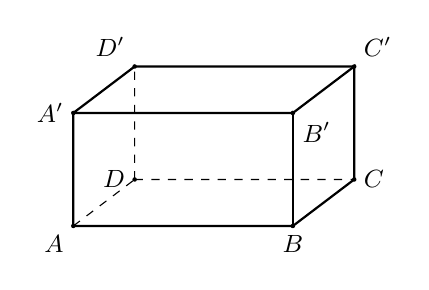
\begin{tikzpicture}[scale=0.82,>=stealth,font=\small]
  \coordinate (A) at (0,0);
  \coordinate (B) at (3.4,0);
  \coordinate (C) at (4.35,0.72);
  \coordinate (D) at (0.95,0.72);
  \coordinate (Ap) at (0,1.75);
  \coordinate (Bp) at (3.4,1.75);
  \coordinate (Cp) at (4.35,2.47);
  \coordinate (Dp) at (0.95,2.47);
  \draw[thick] (A)--(B)--(C)--(Cp)--(Bp)--(Ap)--cycle;
  \draw[thick] (Ap)--(Dp)--(Cp);
  \draw[thick] (A)--(Ap) (B)--(Bp);
  \draw[dashed] (A)--(D) (D)--(C) (D)--(Dp);
  \fill (A) circle (1pt) node[below left] {$A$};
  \fill (B) circle (1pt) node[below] {$B$};
  \fill (C) circle (1pt) node[right] {$C$};
  \fill (D) circle (1pt) node[left] {$D$};
  \fill (Ap) circle (1pt) node[left] {$A'$};
  \fill (Bp) circle (1pt) node[below right] {$B'$};
  \fill (Cp) circle (1pt) node[above right] {$C'$};
  \fill (Dp) circle (1pt) node[above left] {$D'$};
\end{tikzpicture}
\end{center}
\nopagebreak[4]
\Needspace{5\baselineskip}
（7） 方程

\nopagebreak[4]
\[
\log_2(x-3)=\log_4(5-x)
\]

的解是 $\underline{\hspace{4em}}$。

\Needspace{5\baselineskip}
（8） 已知 $\sin\alpha=\dfrac13$，$2\pi<\alpha<3\pi$，那么

\nopagebreak[4]
\[
\sin\frac\alpha2+\cos\frac\alpha2=
\]

 $\underline{\hspace{4em}}$。

\Needspace{5\baselineskip}
（9） 计算

\nopagebreak[4]
\[
\lim_{n\to\infty}\left(\frac1{n^2}+\frac4{n^2}+\frac7{n^2}+\cdots+\frac{3n-2}{n^2}\right)
\]

 $\underline{\hspace{4em}}$。

（10） 抛物线 $y=4x^2-4x$ 的准线方程是 $\underline{\hspace{4em}}$。

\end{question}
\begin{question}
\gkti{2}

二、选择题

（1） 若 $\alpha$ 是第四象限的角，则 $\pi-\alpha$ 是\mbox{（　　）}

（A）第一象限的角　　（B）第二象限的角

（C）第三象限的角　　（D）第四象限的角

（2） 以点 $A(-5,4)$ 为圆心，且与 $x$ 轴相切的圆的标准方程是\mbox{（　　）}

（A）$(x+5)^2+(y-4)^2=16$

（B）$(x-5)^2+(y+4)^2=16$

（C）$(x+5)^2+(y-4)^2=25$

（D）$(x-5)^2+(y+4)^2=25$

（3） 若 $a<b<0$，则下列不等关系中不能成立的是\mbox{（　　）}

（A）$\frac1a>\frac1b$　　（B）$\frac1{a-b}>\frac1a$

（C）$|a|>|b|$　　（D）$a^2>b^2$

（4） 两排座位，第一排有 3 个座位，第二排有 5 个座位。若 8 名学生入座（每人一个座位），则不同坐法的种数是\mbox{（　　）}

（A）$C_8^5C_8^3$　　（B）$P_2^1C_8^5C_8^3$

（C）$P_8^5P_8^3$　　（D）$P_8^8$

（5） 设 $z_1,z_2$ 为复数，那么“$z_1^2+z_2^2=0$”是“$z_1,z_2$ 同时为零”的\mbox{（　　）}

（A）充分不必要条件　　（B）必要不充分条件

（C）充分必要条件　　（D）既不充分又不必要条件

（6） 下面四个函数中为奇函数的是\mbox{（　　）}

（A）$y=x^2\sin\left(x+\frac\pi2\right)$

（B）$y=x^2\cos\left(x+\frac\pi4\right)$

（C）$y=\cos(\operatorname{arc\,ctg}x)$

（D）$y=\operatorname{arc\,ctg}(\sin x)$

（7） 下列四个命题中的真命题是\mbox{（　　）}

（A）若直线 $l$ 与平面 $\alpha$ 内两条平行直线垂直，则 $l\perp\alpha$。

（B）若平面 $\alpha$ 内两条直线与平面 $\beta$ 内两条直线分别平行，则 $\alpha\parallel\beta$。

（C）若平面 $\alpha$ 与二面角 $\beta$-$MN$-$\gamma$ 的棱 $MN$ 交于点 $A$，与二面角的面 $\beta$、面 $\gamma$ 分别交于 $AB$、$AC$，则 $\angle BAC\le90^\circ$。

（D）以上三个命题都是假命题。

（8） 要得到函数 $y=\cos\left(2x-\dfrac\pi4\right)$ 的图象，只需将函数 $y=\sin 2x$ 的图象\mbox{（　　）}

（A）向左平移 $\dfrac\pi8$ 个单位　　（B）向右平移 $\dfrac\pi8$ 个单位

（C）向左平移 $\dfrac\pi4$ 个单位　　（D）向右平移 $\dfrac\pi4$ 个单位

（9） 设直角三角形 $\triangle ABC$ 的直角边 $BC=a$、$AC=b$，斜边 $AB=c$，且 $a<b$。分别以直线 $BC$、$AC$ 和 $AB$ 为轴将直角三角形绕轴旋转一周，所得三个旋转体的体积分别记为 $V_1,V_2,V_3$，那么 $V_1,V_2,V_3$ 间的大小关系是\mbox{（　　）}

（A）$V_3>V_1>V_2$　　（B）$V_1>V_2>V_3$

（C）$V_1>V_3>V_2$　　（D）$V_2>V_1>V_3$

（10） 下列参数方程（$t$ 是参数）中与方程 $y^2=x$ 表示同一曲线的是\mbox{（　　）}

（A）$\begin{cases}x=t,\\y=t^2;\end{cases}$
　（B）$\begin{cases}x=\sin^2t,\\y=\sin t;\end{cases}$

（C）$\begin{cases}x=t,\\y=\sqrt{|t|};\end{cases}$
　（D）$\begin{cases}x=\dfrac{1-\cos2t}{1+\cos2t},\\y=\operatorname{tg}t.\end{cases}$

\end{question}
\begin{question}
\gkti{3}

三、解答题

\Needspace{5\baselineskip}
（1） 求

\nopagebreak[4]
\[
\cos\left(2\operatorname{arc\,tg}\sqrt6+\frac\pi3\right)
\]

的值。

\Needspace{5\baselineskip}
（2） 求函数

\nopagebreak[4]
\[
y=\sqrt{2+\log_{1/2}x}+\sqrt{\operatorname{tg}x}
\]

的定义域。

（3） 在直角坐标系 $xOy$ 中，过点 $P(-3,4)$ 的直线 $l$ 与直线 $OP$ 的夹角为 $45^\circ$，求直线 $l$ 的方程。

（4） 在 $(1-x^2)^{20}$ 的展开式中，如果第 $4r$ 项和第 $r+2$ 项的二项式系数相等，

（1） 求 $r$ 的值；

（2） 写出展开式中的第 $4r$ 项和第 $r+2$ 项。

\Needspace{0.4\textheight}
\end{question}
\begin{question}
\gkti{4}

\Needspace{5\baselineskip}
四、如图，设点 $A\text{、}B$ 分别在二面角 $M$-$PQ$-$N$（平面角为锐角）的两个面 $N\text{、}M$ 上，直线 $AB$ 与面 $M\text{、}N$ 所成的角分别为 $\alpha\text{、}\beta$。过点 $A\text{、}B$ 分别作棱 $PQ$ 的垂线 $AE\text{、}BF$，垂足为 $E\text{、}F$。求证：

\nopagebreak[4]
\[
\frac{AE}{BF}=\frac{\sin\alpha}{\sin\beta}\text{。}
\]
\nopagebreak[4]
\begin{center}% 1989 年上海卷第四题：二面角及垂足示意；图形不表示精确角度或比例
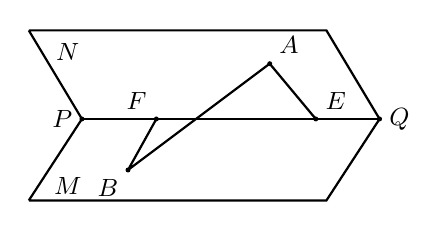
\begin{tikzpicture}[scale=0.9,>=stealth,font=\small]
  \coordinate (P) at (0,0);
  \coordinate (Q) at (4.2,0);
  \coordinate (N1) at (-0.75,1.25);
  \coordinate (N2) at (3.45,1.25);
  \coordinate (M1) at (-0.75,-1.15);
  \coordinate (M2) at (3.45,-1.15);
  \coordinate (A) at (2.65,0.78);
  \coordinate (B) at (0.65,-0.72);
  \coordinate (E) at (3.3,0);
  \coordinate (F) at (1.05,0);
  \draw[thick] (N1)--(N2)--(Q) (P)--(N1);
  \draw[thick] (M1)--(M2)--(Q) (P)--(M1);
  \draw[thick] (P)--(Q);
  \draw[thick] (A)--(B) (A)--(E) (B)--(F);
  \fill (P) circle (1pt) node[left] {$P$};
  \fill (Q) circle (1pt) node[right] {$Q$};
  \fill (A) circle (1pt) node[above right] {$A$};
  \fill (B) circle (1pt) node[below left] {$B$};
  \fill (E) circle (1pt) node[above right] {$E$};
  \fill (F) circle (1pt) node[above left] {$F$};
  \node at (-0.2,0.95) {$N$};
  \node at (-0.2,-0.95) {$M$};
\end{tikzpicture}
\end{center}
\nopagebreak[4]
\end{question}
\begin{question}
\gkti{5}

\Needspace{5\baselineskip}
五、设复数集合

\nopagebreak[4]
\[
M=\{z\mid |z-2+i|\le2,\ z\in\mathbb C\}\cap\{z\mid |z-2-i|=|z-4+i|,\ z\in\mathbb C\}
\]

（1） 试在复平面内作出表示集合 $M$ 的图形，并说出图形的名称；

（2） 求集合 $M$ 中元素 $z$ 的辐角主值的范围；

（3） 求集合 $M$ 中元素 $z$ 的模的范围。

\end{question}
\begin{question}
\gkti{6}

\Needspace{5\baselineskip}
六、已知等比数列 $\{a_n\}$ 的首项 $a_1>0$，公比 $q>-1$ 且 $q\ne0$。设数列 $\{b_n\}$ 的通项

\nopagebreak[4]
\[
b_n=a_{n+1}+a_{n+2}\qquad(n\in\mathbb N)
\]

数列 $\{a_n\}$、$\{b_n\}$ 的前 $n$ 项和分别记为 $A_n\text{、}B_n$。试比较 $A_n$ 与 $B_n$ 的大小。

\end{question}
\begin{question}
\gkti{7}

\Needspace{5\baselineskip}
七、$F$ 是定点，$l$ 是定直线，点 $F$ 到直线 $l$ 的距离为 $p$（$p>0$）。点 $M$ 在直线 $l$ 上滑动，动点 $N$ 在 $MF$ 的延长线上，且满足条件

\nopagebreak[4]
\[
\frac{|FN|}{|MN|}=\frac1{|MF|}\text{。}
\]

（1） 求动点 $N$ 的轨迹；

（2） 求 $|MN|$ 的最小值。

\end{question}